\graphicspath{{./figures}}

\section{Antenna Theory}\label{sec:antenna_theory}

This section covers a very brief review of different types of antennas in literature, as well as how to practical feed these antennas with a transmission line, and a summary of their varying performances.

\subsection{Types}\label{sec:antenna_types}
There are various antenna types to consider for a satellite communication system. A highly-customized antenna design is out of the scope of this project, and therefore only common designs with tunable parameters, or existing designs in literature, will be considered. Ultimately, the following characteristics will be used to compare the various options:
\begin{itemize}
    \item Radiation pattern (qualitative shape)
    \item Gain (relative to an \textit{isotropic} source) 
    \item Bandwidth (relative to resonant frequency)
    \item Beamwidth (angular width of \textit{main lobe})
    \item Dimensions
\end{itemize}

\subsubsection{Half-Wavelength Dipole}
\begin{figure}[!htb]
  \centering
  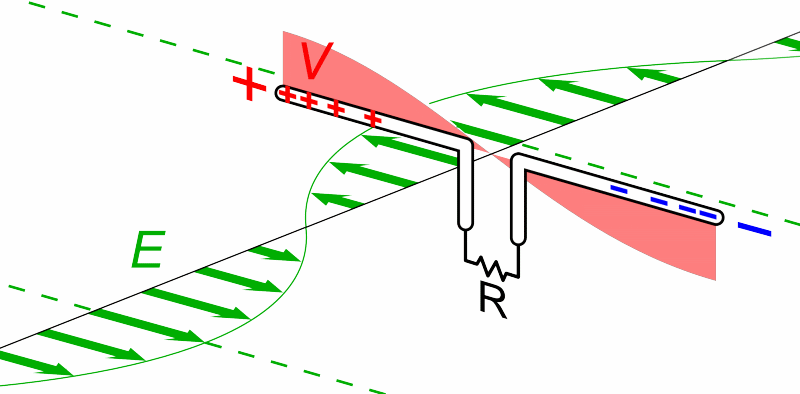
\includegraphics[width=0.4\textwidth]{dipole}
  \caption{Dipole Antenna Illustration \cite{site-designingDipole}}
  \label{fig:dipole}
\end{figure}

The half-wavelength ($0.5 \lambda$) dipole anntenna is arguably the simplest and most common type of antenna. It consists of two conductive elements operating in opposite phase, as depicted in Figure \ref{fig:dipole}. It is considered \textit{omni-directional} i.e. it radiates equally in a given plane. These antennas have a relatively low gain of around 2.15 dBi \cite{site-antennaTheory}. Further, they do not radiate in the direction tangential to their conductor.

\subsubsection{General Dipole}
Dipole antennas can, in general, be any length. However, a change in length results in a change in the antenna's characteristics. In general, smaller antennas result in lower gain and lower efficiency, but a larger beamwidth at the resonant frequency. The obvious advantage of these designs is that the size of the dipole can be decreased. However, if size is a constraint, \textit{monopole} antennas are generally employed.

\subsubsection{Quarter-Wave Monopole}\label{monopole}
The working principle of a classic monopole antenna makes use of the electromagnetic theory of \textit{imaging}. If an infinite ground plane or Perfect Electrical Conductor (PEC) is placed below one half of a $0.5 \lambda$ dipole antenna, then, since the PEC holds the constraint that the tangential electric field is zero across its boundary, an equal but opposite electromagnetic wave is "induced" due to the incident wave. This wave "appears" to have come from an equal but oppositely polarized "image" source, hence removing the need for the second half of the dipole to be present.

These antennas are extremely useful when size is a constraint, however have the disadvantage of requiring a ground plane. A \textit{whip} antenna is a form of monopole antenna designed to be flexible so that it does not break as easily, and is often placed inside a plastic enclosure, as in Figure \ref{fig:whip}. \cite{site-antennaTheory}

\begin{figure}[!htb]
  \centering
  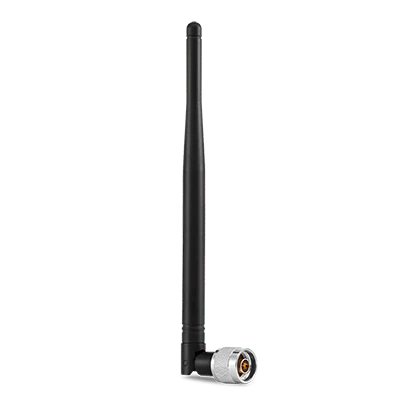
\includegraphics[width=0.3\textwidth]{whip}
  \caption{Whip Antenna in Plastic Housing}
  \label{fig:whip}
\end{figure}

\subsubsection{Helical}
\begin{figure}[!htb]
  \centering
  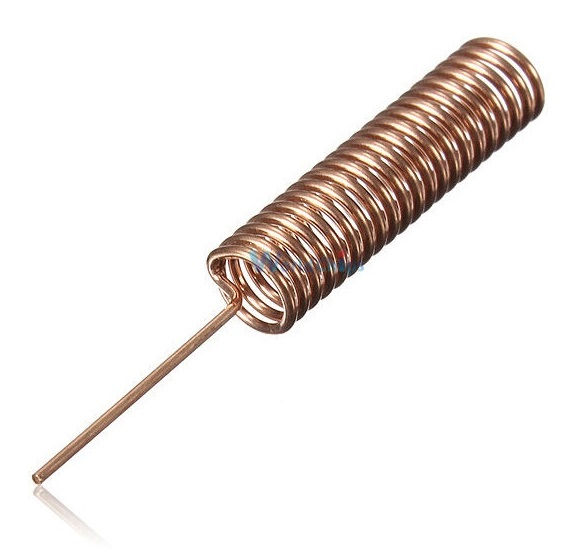
\includegraphics[width=0.2\textwidth]{helical_uni}
  \caption{Helical, Unidirectional Antenna}
  \label{fig:helical_uni}
\end{figure}

Helical antennas are coiled windings of wire, where the circumference of the coil has some relationship with the desired wavelength. Commonly, a circumference of $C = 1.0 \lambda$ is used for \textit{unidirectional} variants. In this case, a ground plane is required (referring to the theory of imaging in Section \ref{monopole}). The ground plane can also be \textit{cupped} (i.e. extended as an open cylinder) for additional directivity \cite{textbook-antennaTheoryAnalysisDesign}. \textit{Omni-directional} variants are also possible, which have a circumference much smaller than the operating wavelength, and do not require a ground plane \cite{site-helixAntennas}. When $C \approx \lambda$, the antenna is said to be operating in \textit{axial mode}. Conversely, when $C << \lambda$, the antenna operates in \textit{normal mode}. Figure \ref{fig:helical_uni} depicts a 21-turn antenna designed to operate in normal mode.

Helical antennas have several design parameters that influence the antennas characteristics, such as number of turns ($n$), wire width ($wd$), and spacing between turns ($S$). A spacing of $0.20 \lambda < S < 0.25 \lambda$ is recommended, however smaller spacings of $0.10 \lambda < S < 0.20$ are commonly used \cite{site-helicalCalculator}. They also are able to receive either linear or circularly polarized signals, making them more flexible. Lastly, since they can be designed with an arbitrarily small or large number of turns, and they have a large operating bandwidth, they can be made smaller than other alternatives.

\subsubsection{Patch}
A \textit{patch} antenna (collequially known as a \textit{PCB} antenna) is simply a rectangular PCB trace sized correctly to allow for radiation. Typically, a simple square or rectangular shape can be used. They allow for small profiles at the cost of efficiency \cite{site-antennaTheory}, and can be integrated onto a PCB using normal trace techniques.

\subsubsection{Array}
In general, multiple antennas can be combined in what is known as an \textit{array} configuration. This allows complete manipulation of the design, by virtue of \textit{constructive} and \textit{destructive} interference of the electromagnetic waves. This can allow for either an increase, or decrease in directivity. Common variations of this concept reside in \textit{Yagi-Uda} and \textit{Patch Array} antennas. \cite{site-antennaTheory}

\subsubsection{Yagi-Uda}
\begin{figure}[!htb]
  \centering
  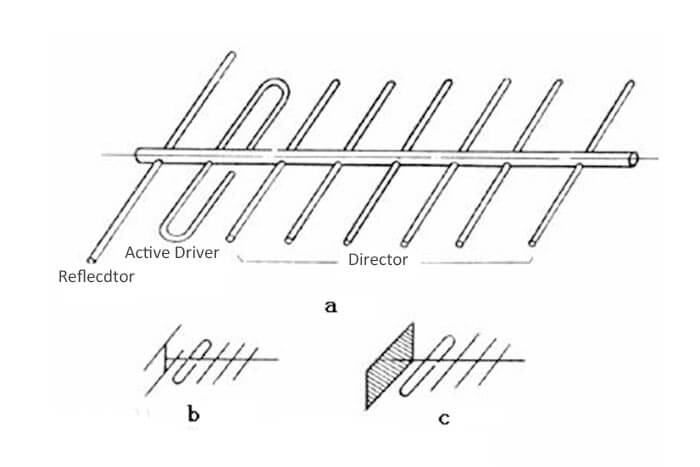
\includegraphics[width=0.4\textwidth]{yagi}
  \caption{Yagi-Uda Antenna \cite{site-icantennasYagi}}
  \label{fig:yagi}
\end{figure}
Although not strictly an antenna array, \textit{Yagi-Uda} antennas are one of the most popular directive antennas. A given number of conductors are stacked in a specific configuration as show in  Figure \ref{fig:yagi}. This ultimately "steers" the electromagnetic waves using the concept of interference. Only one of the conductors in the array is actually fed with the signal - the rest are merely \textit{passive} elements used for increasing the directivity.

\subsubsection{Microstrip}
\begin{figure}[!htb]
  \centering
  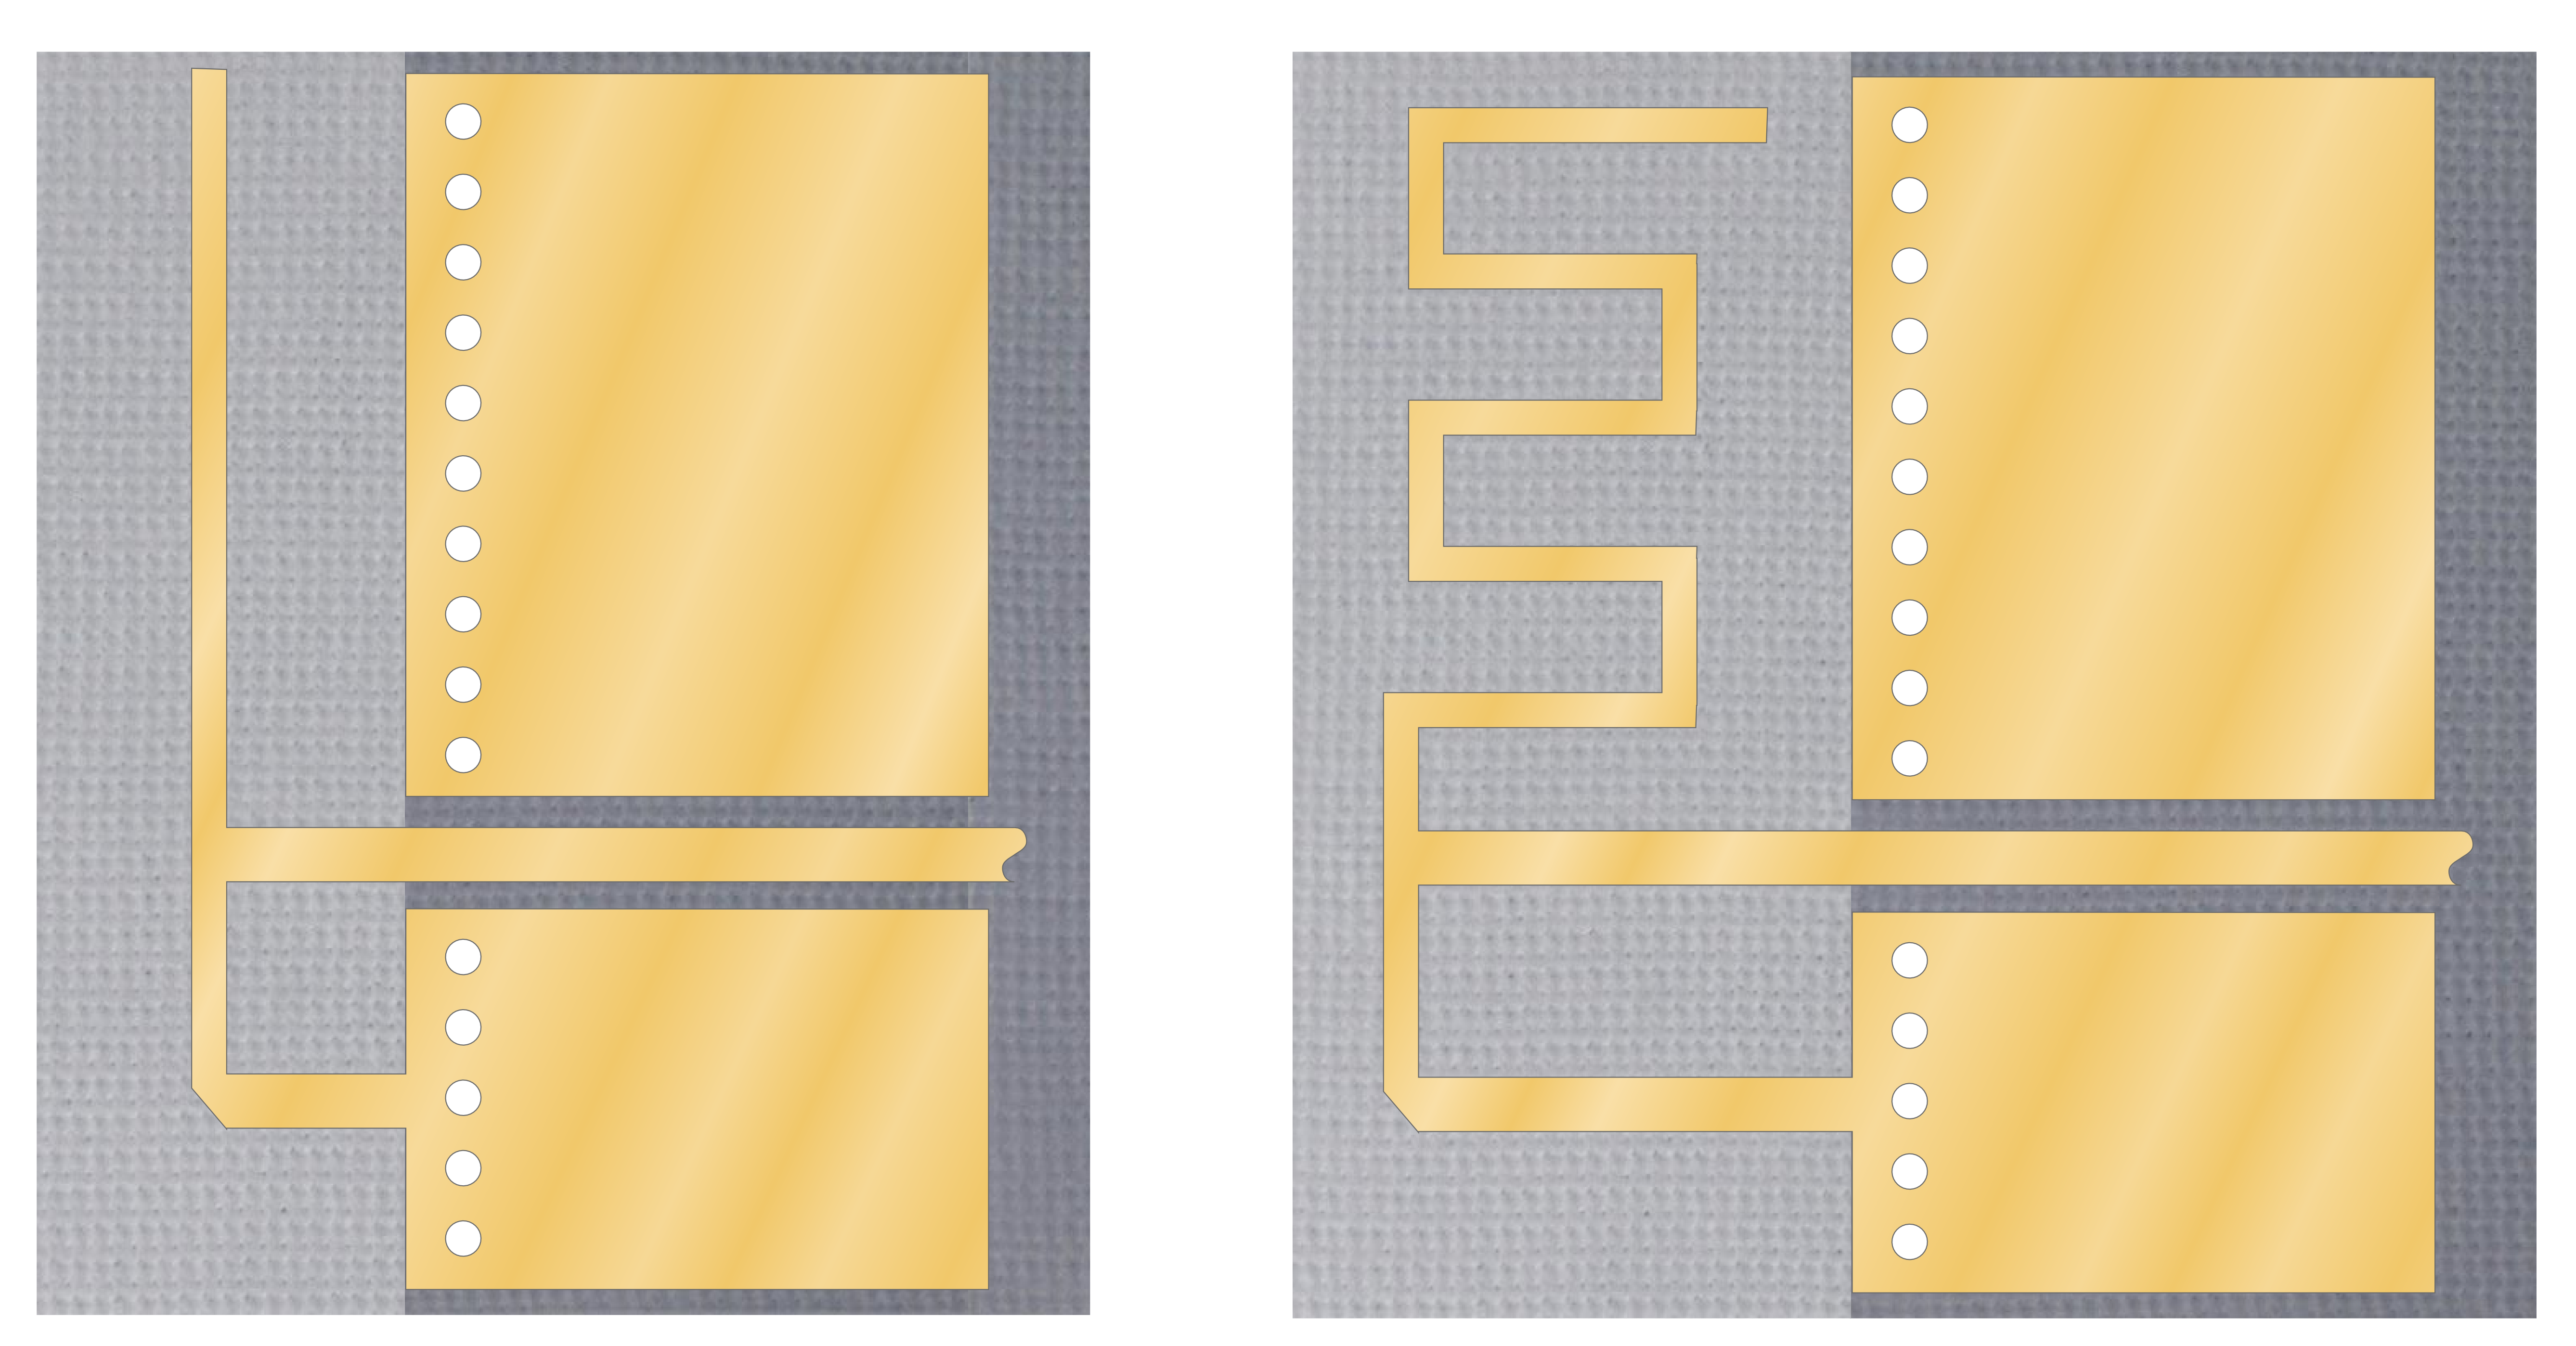
\includegraphics[width=0.3\textwidth]{invertedF}
  \caption{Inverted-F Microstrip Antennas \cite{site-invertedFAntenna}}
  \label{fig:invertedF}
\end{figure}
\textit{Microstrip} antennas generally refer to any planar, PCB antenna. They can be considered a generalization of a patch antenna. Many designs exist (often derived from non-planar antennas) due to their flexible nature. This allows for a diverse selection of desired characteristics. A few examples include:
\begin{itemize}
  \item A \textit{patch array}, which has increased directivity.
  \item An \textit{inverted-F} design, which has a small form factorer and a nearly 3D omni-directional radiation pattern.
  \item A \textit{ring antenna}, which is unidirectional, and has an even smaller form factor than the inverted-F antenna \cite{paper-lowProfileRingAntenna}.
  \item A \textit{helical patch} antenna, which is simply a "zig-zag" helix shape flattened onto a PCB.
\end{itemize}

A multi-frequency inverted-F design is illustrated in Figure \ref{fig:invertedF}.

\subsection{Feedline}
In general, \textit{feeding} an antenna is more complicated than simply connecting the amplifier's positive and negative terminals to the antenna's terminals. A $\SI{50}{\ohm}$ characteristic impedance is often used in RF systems. Since each antenna has a unique \textit{input impedance} which is generally different from this value, it must be \textit{matched} appropriately for optimal performance.

A general, antenna-agnostic narrow-band technique for antenna impedance matching is to employ a "lumped element" matching circuit consisting mainly of inductors and capacitors. The most common example of this is an L-section, with exactly one capacitor and inductor. A few well-known techniques for a number of the antennas in Section \ref{sec:antenna_types} are reviewed below.

\subsubsection{Half-Wavelength Dipole}
A half-wavelength dipole antenna has an input impedance of around $\SI{73}{ohms}$, varying only due to the wire diameter used. A common method to reduce this impedance to $\SI{50}{ohms}$ is simply to reduce the length of the dipole. In this case, a $\SI{50}{ohms}$ match occurs at between $\SI{0.42}{\lambda}$ and $\SI{0.44}{\lambda}$. \cite{textbook-antennaTheoryAnalysisDesign}

\subsubsection{Helical}\label{sec:helical_matching}
The input impedance of a helical antenna varies between 100 and 200 ohms. A common method to reduce this impedance is for the first quarter turn of the helix to be in the form of a conductive strip, and for the \textit{pitch angle} of this section to be close to zero \cite{textbook-antennaTheoryAnalysisDesign}. The height above the ground plane can then be varied to match the antenna appropriately, with the following equation approximately providing an approximate $\SI{50}{\ohm}$ match \cite{textbook-antennaTheoryAnalysisDesign}:
$$h = \frac{w}{\frac{377}{\sqrt{\epsilon_r} Z_0} - 2}$$

\subsection{Summary}
The following table presents a general summary of the investigated antennas. A qualitative comparison of the results have been presented (from general consensus in literature) to aid in the design phase. Note that a \textit{narrow} beamwidth general corresponds to a \textit{unidirectional} antenna (and wide for omni-directional) and therefore this characteristic has not been included in the table.

\begin{table}[!htb]
  \centering
  \hspace*{-2cm}
  \renewcommand{\arraystretch}{1.2}
  \begin{tabular}{ |c|c|c|c|c|c| }
  \hline
  \textbf{Type} & \textbf{Gain (dBi)} & \textbf{Radiation} & \textbf{Bandwidth} & \textbf{Size} \\ \hline
  $0.5 \lambda$ Dipole & 2.15 & Omnidirectional & Medium & Medium \\ \hline
  Monopole & 5.15 & Omnidirectional & Small & Small \\ \hline
  Helical & $<20$ & Either & Large (50 - 60\%) & Small-Medium \\ \hline
  Microstrip & $<10$ & Either & Small-Medium & Small \\ \hline
  Yagi-Uda & $<40$ & Unidirectional & Small & Large \\ \hline
  \end{tabular}
  \caption{Qualitative Comparison of Antenna Characteristics \cite{site-antennaTheory}}
  \label{tab:antenna_characteristics}
\end{table}